The device fabrication consists of four main processes. Included in these processes are various lithography steps, evaporation of different metals, wet etching and deposition of silicon nitride as an anti-reflective coating. First, one part of the desired antenna structure is imprinted on a wafer through contact lithography. The photoconductor is dipped into hydrogen chloride (HCl) and the first metal deposition step with chromium and gold is carried out. Then, mesa lithography and mesa etching is applied. Another lithography step for the rest of the antenna structure is executed, followed by the deposition of NiCr. In the end, an anti-reflective coating is deposited. 

\section{CrAu Structure Lithography and Deposition of CrAu}

\begin{figure}[!]
    \centering
    \begin{subfigure}[b]{0.21\textwidth}
        \centering
        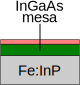
\includegraphics[width=\textwidth]{figures/Fabrication/fab1_1.pdf}
        \caption{\centering}
        \label{fig:fab11}
    \end{subfigure}
    \hfill
    \begin{subfigure}[b]{0.21\textwidth}
        \centering
        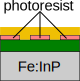
\includegraphics[width=\textwidth]{figures/Fabrication/fab1_2.pdf}
        \caption{\centering}
        \label{fig:fab12}
    \end{subfigure}
    \hfill
    \begin{subfigure}[b]{0.21\textwidth}
        \centering
        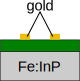
\includegraphics[width=\textwidth]{figures/Fabrication/fab1_3.pdf}
        \caption{\centering}
        \label{fig:fab13}
    \end{subfigure}
    \caption{Schematic diagram depicting the principle steps of structure lithography and metal deposition. (a) The wafer is covered in AZ 5214E photoresist. (b) UV exposure leaves behind a patterned photoresistive structure. A metal layer is deposited through metal evaporation on top of the photoresistive layer. (c) Lift-off is performed to get rid of the excess metal. Left behind is only the metal in contact with the semiconducting material.}
\end{figure}

A lithography mask is fabricated containing the desired antenna structures. A \num{7} $\times$ \num{8} \si{\milli\meter} sample of an InGaAs photoconductor, grown on a \num{500} \si{\micro\meter} InP:Fe substrate wafer is cleaved out from the wafer. In the following steps, structures as small as \num{5} \si{\micro\meter} are desired, so good contact and alignment are critical.

First, a fabrication step called zero-leveling is executed. The zero-leveling helps in achieving good contact when applying contact lithography. A thin layer of AZ 5214E image reversal photoresist is deposited onto the sample. By spin coating the sample at 8000 rpm, a uniform layer of photoresist is achieved. 
By soft baking the sample at \num{110} \si{\celsius} for one minute, it is prepared for ultraviolet (UV) exposure. 
The sample is exposed to UV light for \num{35} seconds, before being developed using AZ MIF 726, leaving a \num{5} $\times$ \num{6} \si{\milli\meter} area of photoresist.
A second lithographic step is carried out to define the antenna structures intended to be fabricated from chromium–gold (CrAu). The lithography mask is applied to the sample, which is then exposed to UV light for \num{3} seconds, followed by another soft baking step. A second UV exposure is carried out with five times the initial exposure duration. The sample is developed using AZ MIF 726, leaving behind the patterned antenna structures ready for CrAu deposition. 

The antenna structures are fabricated through metal deposition. Before depositing the metal for the PCAs, the samples are dipped into a 1:1 solution of H\textsubscript{2}O and HCl for \num{15} seconds to remove the oxide layer which forms at the surface. This step greatly improves the adhesion of the deposited metal. In the first metal deposition step, gold structures are deposited on top of a chromium adhesion layer. The antenna electrodes, contact pads and some part of the feeding strip are fabricated by depositing a \num{120} \si{\nano\meter} layer of gold (Au) on top of a \num{20} \si{\nano\meter} layer of Chrome (Cr) via thermal evaporation. Cr is deposited at a rate of $\sim 0.3$ \si{\angstrom}/\si{\s}, Au is deposited at a rate of $\sim 0.8$ \si{\angstrom}/\si{\s}. The Cr-layer improves the contact with the semiconducting material. After completing the metal deposition, the sample is placed in acetone and lift-off is performed. This way we get rid of the unwanted metal on our sample. 

An additional annealing step is performed after metal deposition to further improve the metal-semiconductor-contact. Such an annealing process reduces the interface impurities and creates good contact on the atomic scale between the metal and the semiconducting material \cite{tahamtanInvestigationEffectAnnealing2011}. Metal atoms diffuse into the InGaAs, making sure that we get an ohmic contact rather than a Schottky contact. Annealing is performed at a temperature of $\sim 422$ \si{\celsius} for \num{30} seconds under a nitrogen atmosphere at a pressure of \num{2} \si{\milli \bar}.  

\section{Mesa Lithography and Mesa Etching}

A layer of AZ 1518 HS photoresist is deposited onto the sample. Spin coating at 4000 rpm ensures a uniform photoresistive layer. Contact lithography is performed before hard baking the sample covered in photoresist at \num{110} \si{\celsius} for \num{15} minutes. By hard baking the sample, the resist is 
By hard baking the sample, the layer of photoresist is made more resistant to etching.   

The InGaAs photoconductive material is etched from the areas that were not protected by the photoresist layer using 
sulfuric acid (H\textsubscript{2}SO\textsubscript{4}), hydrogen peroxide (H\textsubscript{2}O\textsubscript{2}) and water (H\textsubscript{2}0) mixed in appropriate proportion. We use a ratio of \num{1} \si{\milli \liter} : \num{8} \si{\milli \liter} : \num{50} \si{\milli \liter} respectively. The semi-insulating InP:Fe substrate is left exposed in those areas. 

By mesa etching, the active InGaAs layer is removed from the entire sample except between the electrodes and under the antenna and pads. This process ensures a high resistance with a minimal dark current. A minimal dark current drastically improves the signal-to-noise ratio of the THz signal. 

\begin{figure}[!]
    \centering
    \begin{subfigure}[b]{0.21\textwidth}
        \centering
        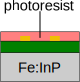
\includegraphics[width=\textwidth]{figures/Fabrication/fab2_1.pdf}
        \caption{\centering}
        \label{fig:fab21}
    \end{subfigure}
    \hfill
    \begin{subfigure}[b]{0.21\textwidth}
        \centering
        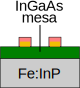
\includegraphics[width=\textwidth]{figures/Fabrication/fab2_2.pdf}
        \caption{\centering}
        \label{fig:fab22}
    \end{subfigure}
    \hfill
    \begin{subfigure}[b]{0.21\textwidth}
        \centering
        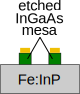
\includegraphics[width=\textwidth]{figures/Fabrication/fab2_3.pdf}
        \caption{\centering}
        \label{fig:fab23}
    \end{subfigure}
    \caption{Schematic diagram depicting the principle steps of structure lithography and metal deposition. (a) The wafer is covered in AZ 5214E photoresist. (b) UV exposure leaves behind a patterned photoresistive structure. A metal layer is deposited through metal evaporation on top of the photoresistive layer. (c) Lift-off is performed to get rid of the excess metal. Left behind is only the metal in contact with the semiconducting material.}
\end{figure}


\section{NiCr Structure Lithography and Deposition of NiCr}

This step is similar to the metal deposition of Au and Cr. The desired structures are imprinted onto the sample through photo-lithography. The imprinted structures are the missing parts of the feeding strips connecting antenna pads and electrodes. Good contact between the NiCr-strip and the AuCr-strip is vital. Otherwise, THz performance will decrease drastically. We spin coat the sample with nLof 2035 at \num{4000} rpm. The sample is soft baked, exposed to UV light and developed using AZ MIF 726. Left behind are the missing parts of the antenna feeding strips, ready for NiCr deposition.

A \num{80}/\num{20} NiCr alloy is deposited onto the sample using flash evaporation. Flash evaporation of \num{80}/\num{20} NiCr involves the rapid heating of the alloy in an evacuated environment (around $10^{-9}$ \si{\bar}). NiCr has a high melting point around \num{1450} \si{\celsius}. The alloy has to be heated rapidly to avoid clumps and bulk melting, assuring a thin, uniform NiCr layer on top of the sample. Constantly adjusting the feed rate of the alloy also helps in avoiding bulking. Ideally, the deposition rate should be kept as low as possible. In this work, the rate was kept at around \num{0.3} \si{\angstrom}/\si{\s}. As Nickel and chromium have slightly different melting temperatures it is also vital to make sure that the two metals are evaporated at equal rates.The 80/20 ratio is important to ensure that the NiCr alloy’s conductivity remains within the desired range. Upon reaching its evaporation temperature, the NiCr vaporizes, travels through the vacuum and accumulates on the sample surface.
\section{Anti-Reflection Coating Deposition}
\begin{wrapfigure}{r}{0.4\textwidth} % r = right side, 50% of text width
    \centering
    
\includegraphics[width=0.39\textwidth]{figures/Fabrication/PCA_after_NiCr.pdf}
    \captionsetup{width=0.375\textwidth} % caption matches image width
    \caption{Schematic diagram of PCA cross section after NiCr deposition. The overlaps are idealized.}
    \label{fig:afterFab}
\end{wrapfigure}
An anti-reflection coating (ARC) is deposited above the active region. The ARC layer improves the absorption of the incoming infrared signal in the active region  \cite{chenAntireflectionImplementationsTerahertz2014} and protects the device from external damage. In the simplest implementation, an ARC consists of a single layer having the thickness of an odd multiple of the quarter-wavelength of the incident light: $d \sim k \frac{\lambda}{4}$. The refractive index of the coating material is chosen to be approximately the geometric mean of the indices of the two surrounding media. This choice ensures that the reflections occurring at the two interfaces are equal in magnitude and offset in phase. This leads to destructive interference and, consequently, reduced reflection (see Figure \ref{fig:fabarc}) \cite{paschottaAntireflectionCoatings2005}. 
The ARC is fabricated by growing a silicon nitride (Si\textsubscript{3}N\textsubscript{4}) layer on top of the sample via plasma-enhanced chemical vapor deposition (PECVD). Si\textsubscript{3}N\textsubscript{4} has a refractive index of $n_1 \approx 1.89$. We choose a thickness of $d = \frac{1}{4} \frac{\lambda}{n_1}$ for a wavelength of $\lambda = 1550$ \si{\nano \meter}, resulting  in a Si\textsubscript{3}N\textsubscript{4}-thickness of $d \approx 205$ \si{\nano \meter}. The Si\textsubscript{3}N\textsubscript{4}is deposited at a rate of approx. \num{13.5} \si{\nano \meter/\min}. After depositing the Si\textsubscript{3}N\textsubscript{4}, another layer of AZ 1518 HS photoresist is deposited onto the sample to form the required patterns of the Si\textsubscript{3}N\textsubscript{4} over the substrate. The photoresist covers the antenna’s electrode structure and feeding strip but leaves the pads uncovered. Otherwise, measurement of the received signal would not be possible. Photo-lithography is performed to acquire the needed structures. The Si\textsubscript{3}N\textsubscript{4} is etched out from the unprotected areas, exposing the contacting metal pads attached to the antenna. The etching is performed in a PECVD system in reactive ion etching (RIE) mode, using a carbon tetrafluoride (CF\textsubscript{4}) and oxygen (O\textsubscript{2}) plasma to chemically and physically remove the Si\textsubscript{3}N\textsubscript{4}. The unprotected Si\textsubscript{3}N\textsubscript{4} with a thickness of approx. \num{205}\,\si{\nano \meter} is etched in \num{55}\,\si{\s}. After etching of Si\textsubscript{3}N\textsubscript{4} the photoresist is removed by placing the sample in acetone.

\begin{figure}[!]
    \centering
    \begin{subfigure}[b]{0.21\textwidth}
        \centering
        \includegraphics[height=\textwidth]{figures/Fabrication/ARC_deposition_1.pdf}
        \caption{\centering}
        \label{fig:fabarc1}
    \end{subfigure}
    \hfill
    \begin{subfigure}[b]{0.21\textwidth}
        \centering
        \includegraphics[height=0.95\textwidth]{figures/Fabrication/ARC_deposition_2.pdf}
        \caption{\centering}
        \label{fig:fabarc2}
    \end{subfigure}
    \hfill
    \begin{subfigure}[b]{0.45\textwidth}
        \centering
        \includegraphics[width=\textwidth]{figures/Fabrication/ARC.pdf}
        \caption{\centering}
        \label{fig:fabarc}
    \end{subfigure}
    \caption{Schematic diagram depicting the deposition of an ARC and basic ARC working principle. (a) Silicon nitride deposition using a PECVD machine followed by deposition of a photoresistive layer. The photoresistive layer is transformed into structures covering the active region of the antennas using photo-lithography. (b) The silicon nitride is dry etched using carbon tetrafluoride to create the ARC. (c) Working principle of an ARC: incident light is reflected by the air-ARC interface and the ARC-substrate interface. The reflections destructively interfere. Not to scale.}
\end{figure}

\section{Dimensions of Processed Antennas}

\begin{itemize}
    \item umschreiben 
    \item bilder von antennen aufnehmen !!!
\end{itemize}

\begin{figure}[htbp]
    \begin{subtable}[c]{0.45\textwidth}
        \centering
        \begin{tabular}{l|l|l}
        \toprule
        Sample(s) & l\textsubscript{NiCr} [$\mu m$] & l\textsubscript{CrAu} [$\mu m$] \\
        \midrule
        H5, H9, H10 & 0 & 751.5 \\
        H4 & 5 & 746.5 \\
        H1, H2 & 10 & 741.5 \\
        H6 & 15 & 736.5 \\
        H3, H8 & 70 & 701.5 \\
        H7 & 240 & 511.5 \\
        \bottomrule
        \end{tabular}
        \caption{\centering H-Dipole Dimensions}
        \label{tab:table}
    \end{subtable}
    \hspace{0.1em}
    \begin{subtable}[c]{0.45\textwidth}
        \centering
        \begin{tabular}{l|l|l}
        \toprule
        Sample(s) & l\textsubscript{NiCr} [$\mu m$] & l\textsubscript{CrAu} [$\mu m$] \\
        \midrule
        D1, D6 & 0 & 751.5 \\
        D3, D8 & 70 & 701.5 \\
        D4, D9 & 240 & 511.5 \\
        D5, D10 & 500 & 251.5 \\
        D2, D7 & 721.5 & 30 \\
        \bottomrule
        \end{tabular}
        \caption{\centering I-shaped Dipole Dimensions}
        \label{tab:table}
    \end{subtable}
    \caption{}
    \label{fig:sim_dimensions}
\end{figure}

We present the dimensions of the processed H-Dipole and I-shaped Dipole antennas based on the performed simulations. In total, 11 H-Dipole antennas and 13 I-shaped Dipole antennas are processed, partly differing in geometry. Table \ref{} displays the fabricated antennas and their corresponding dimensions important for this work. All of the processed antennas exhibit a strip width of \num{5}\,\si{\micro \meter}. All read-out pads are fabricated as squares, measuring \num{196}\,\si{\micro \meter} $\times$ \num{196}\,\si{\micro \meter}. The total strip length of H-Dipoles and I-shaped Dipoles measures \num{1900}\,\si{\micro \meter}, resulting in an effective strip length of \num{1508}\,\si{\micro \meter} in between the pads. One exception to this rule is an I-shaped Dipole antenna fabricated without adding any NiCr but with increased effective strip length measuring \num{4508}\,\si{\micro \meter}.

